\documentclass[conference]{IEEEtran}
\IEEEoverridecommandlockouts
% The preceding line is only needed to identify funding in the first footnote. If that is unneeded, please comment it out.
\usepackage{cite}
\usepackage{amsmath,amssymb,amsfonts}
\usepackage{algorithmic}
\usepackage{graphicx}
\usepackage{textcomp}
\usepackage{xcolor}
\def\BibTeX{{\rm B\kern-.05em{\sc i\kern-.025em b}\kern-.08em
    T\kern-.1667em\lower.7ex\hbox{E}\kern-.125emX}}
\begin{document}

\title{Implementation and verification of a data vault\\\Large Storing and Managing Data (Module 06-32245), Autumn 2022}

\author{\IEEEauthorblockN{Ningchen, Zhang, 2437506}
nxz107@student.bham.ac.uk\\%Do not modify this line
\today}
%\and
%\IEEEauthorblockN{2\textsuperscript{nd} Given Name Surname}
%\IEEEauthorblockA{\textit{dept. name of organization (of Aff.)} \\
%Signal Processing, Autumn 2020, Course Research Project\\%Do not modify this line
%author email address}


\maketitle

\begin{abstract}
This project aims to construct a data storage project for medical image data storage and further processing. Distinguishing with traditional database forms, the data vault seeks to separate the data itself from the structural information through a range of methods. The project implements data in the form of files in a data warehouse and only updates the existing data without deleting old data sets.\\
This essay begins with a brief introduction to the concept of a data vault\cite{b1}, including its design philosophy and advantages and disadvantages. This is followed by a description of why chose to use a data vault for this project rather than some other model.The results show that the idea of using data vault in the storage of medical images is feasible and effective. The data vault allows the information to be stored separately in satellite tables, and the use of hashes as primary keys to link the entire model which can reduce the redundant information. And by using a timestamped joint primary key, we can ensure that the data does not conflict, so we do not need to consider deleting any data. Finally, the shortcomings of this project are discussed along with the corresponding ideas for improvement.
Key word: data vault, medical image data storage
\end{abstract}

%\begin{IEEEkeywords}
%component, formatting, style, styling, insert
%\end{IEEEkeywords}

\section{Introduction}\label{sec:Intro}
With the development needs of the society, the traditional relational database or No-relational database can no longer meet all our requirements for data storage, such as query efficiency, data security, etc.Dan Linstedt proposed that data vault modeling does not distinguish between better and insufficient data\cite{b2}, meaning that in a data vault, people focus only on data storage and not on its structure or logical conformity to the target. Unlike other types of databases, such as 3NF schema and star schema, the data vault stores the most recent version of the data, so it is identified by the time it was added to the database and any data that does not fit the definition is removed. This construction model makes it easier to help auditors trace back (for data).% course syllabus;

\begin{itemize}
	\item [1) ] 
	Problem description\\
	The problem requires to use of python and SQL to create a minimally functional Data Vault to store medical imaging data, which is derived from patients with protecting complete privacy.     
	\item [2)]
	Goals\\
    The project needs to achieve the following functions:\\ 1) Construct a data vault to store the data in a logical structure\\ 2) Mining the data from the provided data sets and storing the data.\\ 3) Providing a GUI interface to query the added data. 
	\item [3)]
	Achievements and contribution\\
	At the time of writing the report, the program was only designed to read standard 'CSV' files but not to read and add to dat files. It was limited to handling dataset 1. 
\end{itemize}

\section{State of the art of data on vaults}
Data vault now have a model called data vault 2.0 is a model which provides methodologies for data warehousing projects. It provides a very workable solution to meet the needs of data warehousing projects in terms of both historical traces and audits. The data vault 2.0 can use ETL \cite{b3} process which can quickly respond to changes in business logic or the addition of new data. This process is very useful in this project that is the reason to choose data vault 2.0 as basic reference. However, it is not entirely suitable for this project, but only borrows some ideas from datavault 2.0 for the database design of this project.

\section{Methods}
This section will illustrate the methods used in the project 
\subsection{Tools}\label{AA}
This project uses SQL and python. The specific software; for SQL uses PostgreSQL, which has been most popular in recent years and can run on multiple operating systems such as Windows and Mac. Using PgAdmin 4 to visualize tables and data to check for errors at the time of writing; for python, using pycharm is a powerful compiler.\\
\subsection{Data vault and Data design}
For the data vault model. Hubs are used to record unique keys for business entities that are commonly used in business applications.\cite{b4}The connection between Links and Hubs will record a transaction, part or other relationship with hubs. The details of the hubs recorded in the links, for instance, foreign keys and metadata about the time and source link first loaded. \cite{b5}The data in satellites contain Hub or Link and metadata about when and where the data was loaded.\cite{b6}.In the data vault of this project the hubs tables are most important because hubs are the main structure for a data vault model.Base on the feature of requirements, the following design will satisfy the needs of data vault.
\paragraph{Experiment} Storing the experiment objects in this project.
\paragraph{Factor} Storing the factor which may influence the result.
\paragraph{Treatment} The value of each group's treatment of factor is recorded to control the variable
\paragraph{Group} The experiment will have many different group to conduct experimental controls which makes the experiment more rigorous. In this hub stores group information.
\paragraph{ExperimentalUnit} Storing the unit of each experiment.
\paragraph{Subject} Storing the experiment subject which can be considered as patient
\paragraph{Metadata} Storing the metadata of experiment as array.
\paragraph{Observation} Storing the data includes using time and values.In addition storing the data from which session. 
\paragraph{Session} Session
\begin{figure}[htbp]
	\centering{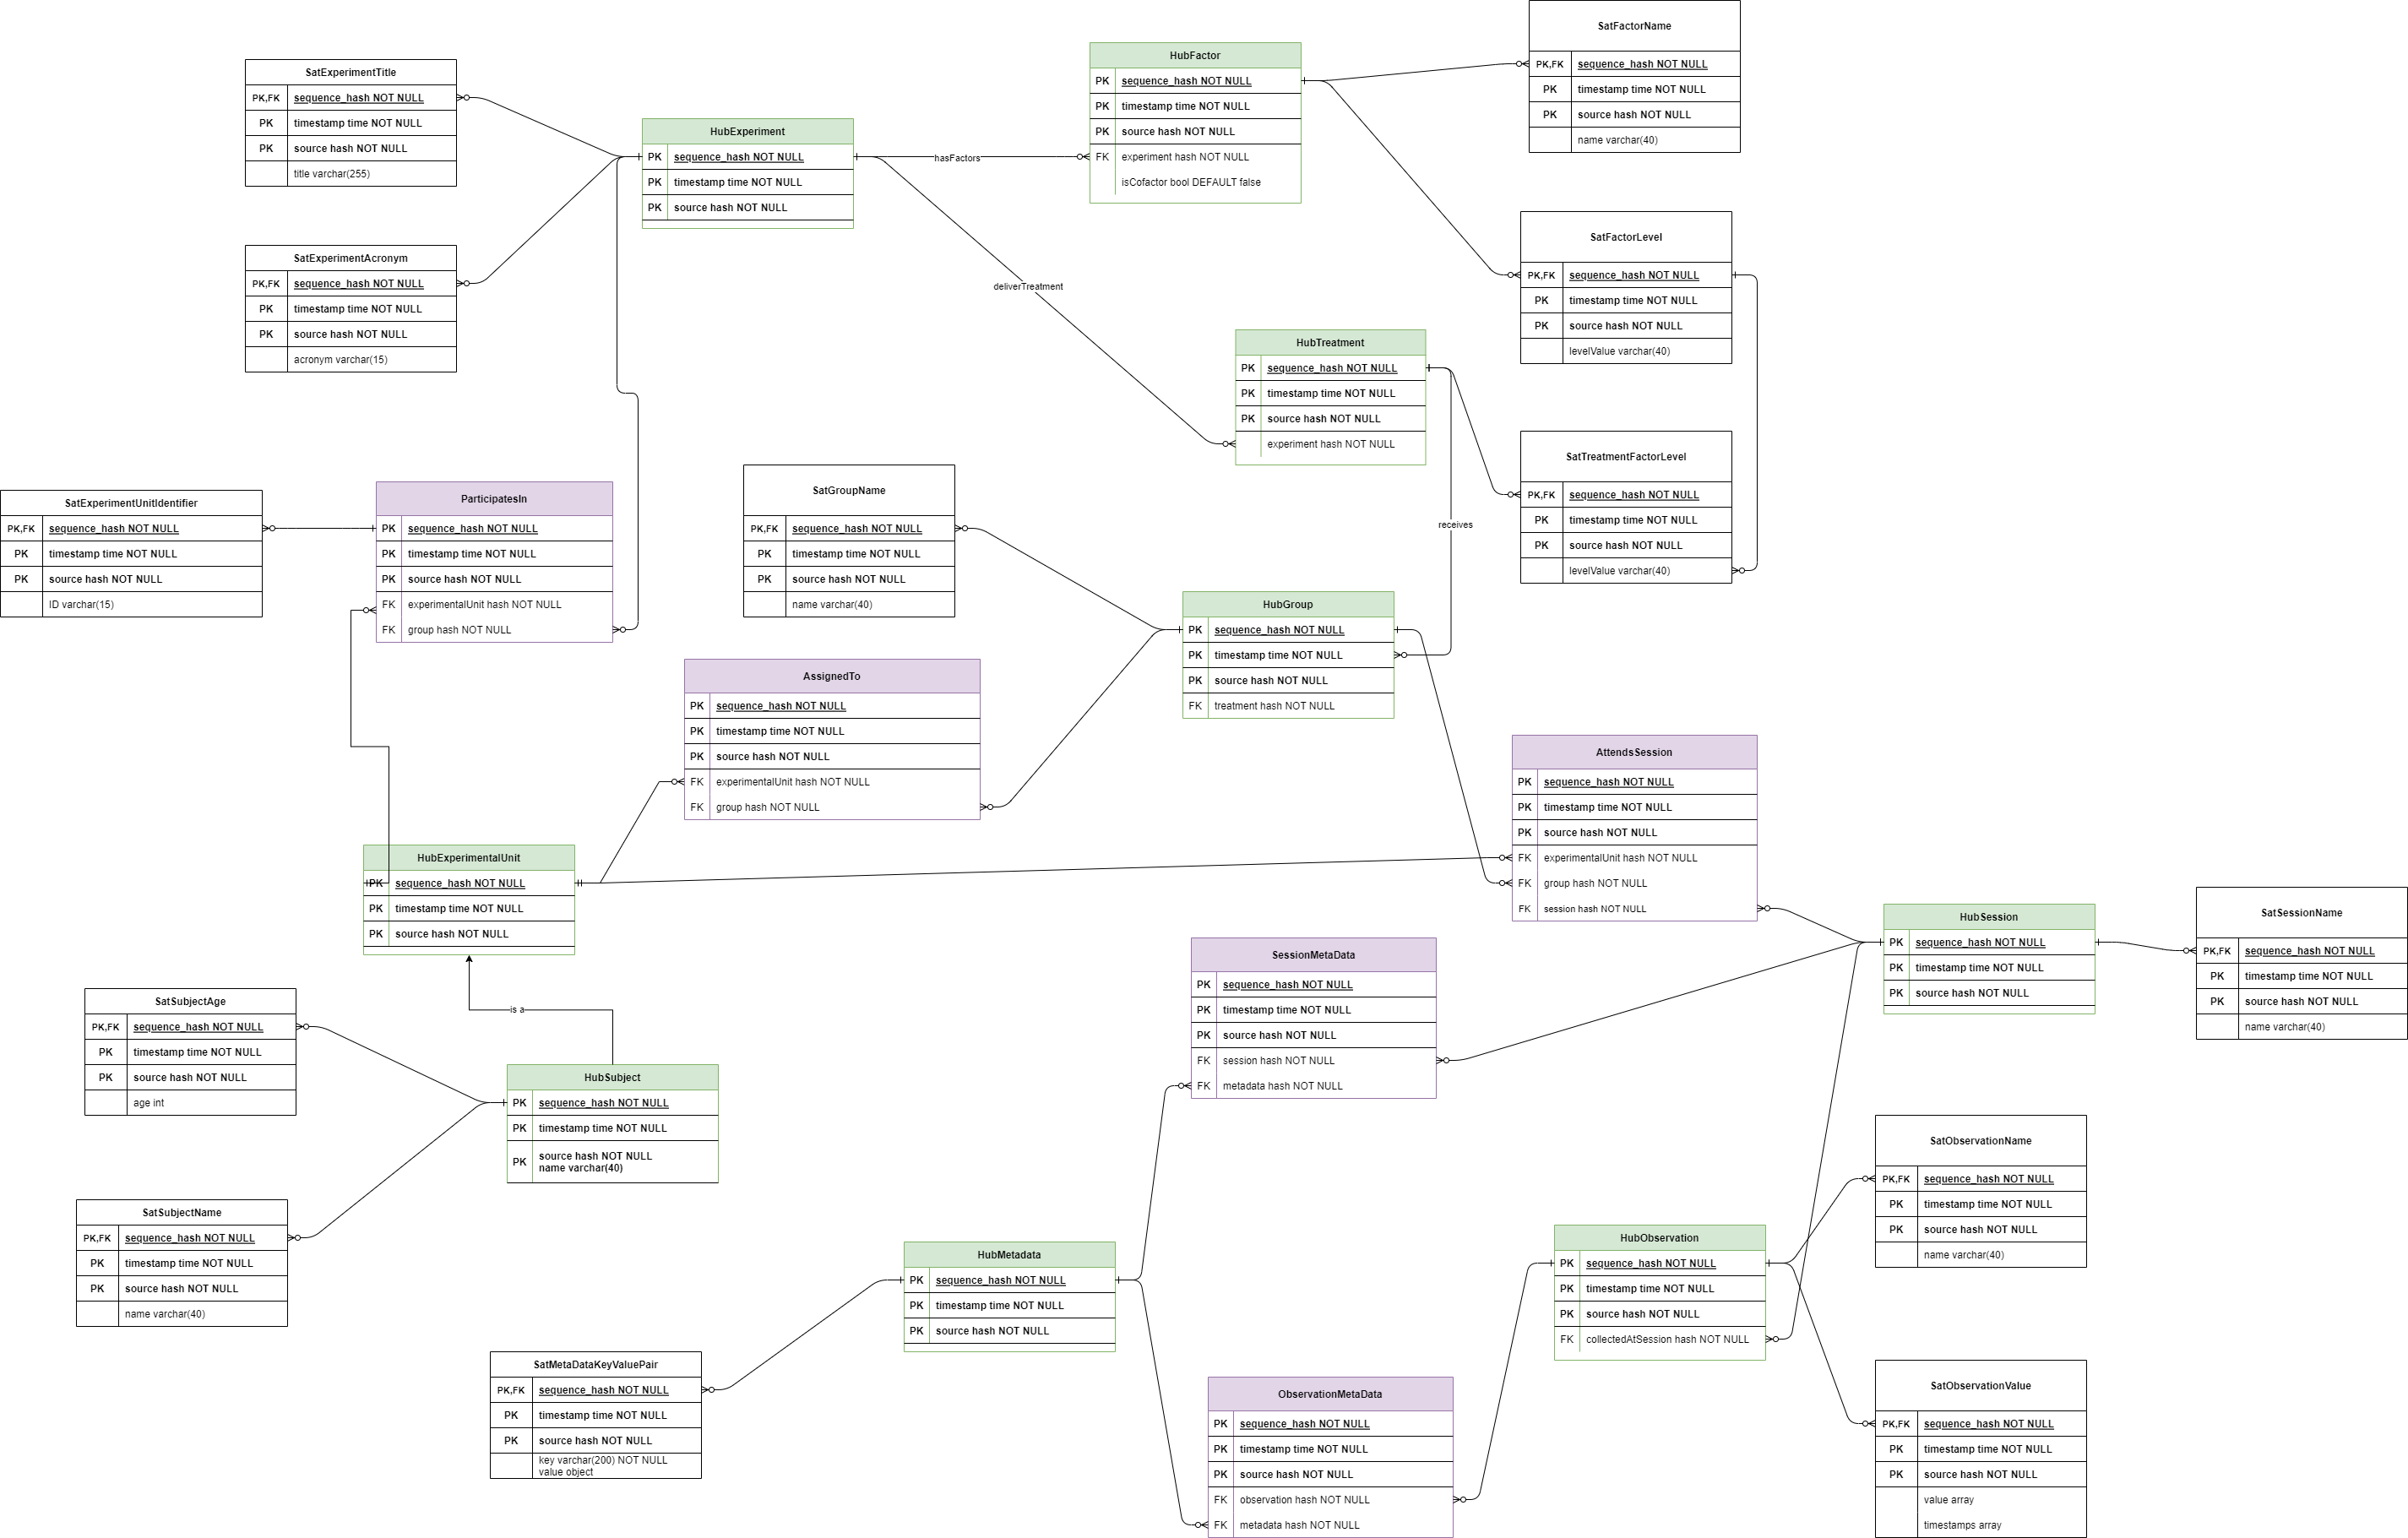
\includegraphics[width=1.0\linewidth]{project.png}}
	\caption{ER-model of data vault}
	\label{project}
\end{figure}
\subsection{main method}
\subsubsection{Psycopg2}
The psycop2 package is a adapter for PostgreSQL database.This package designed for multi-threaded applications that create and destroy a large number of cursors and perform a large number of concurrent "INSERT" or "UPDATEs".The psycopy 2 is created by C which guarantee the effective and safety. In python many data can use directly in PostgreSQL. So using psycop2 to deal with postgreSQL is very effective.\cite{b7}
\subsubsection{Pandas}
Pandas is a very popular package which provides fast,flexible methods to deal with the relational or labeled data like excel files.It has many features but in this project the most important is easy handling of missing data(Empty data)\cite{b8}.In the project uses a unique construct in pandas 'DataFrame' which can help to resolve abnormal data. The data collection process can not guarantee all the data are correct, hence by some function in pandas to deal with it can reduce the impact of bad data on the database.
\subsection{Other important method}\label{AA}
MD5 is a hashing algorithm proposed by Ronald Rivest in 1992. Although its shortcomings have been known in the field of cryptographic security\cite{b9}. In this project, our hash values are intended to ensure no conflicts between primary keys, as the project requirements only update the data instead of delete it. Therefore using the md5 algorithm makes it simple to achieve this. Similar values can result in wildly different outputs that preventing the primary key from failing to insert the data due to a conflict. Python provides a library that allows us to implement the md5 algorithm easily, which is one of the reasons for choosing md5 to calculate the hash value.
\begin{figure}[htbp]
	\centering{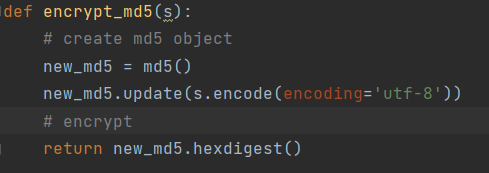
\includegraphics[width=1.0\linewidth]{md5.png}}
	\caption{Md5 in python}
	\label{md5}
\end{figure}

\section{Result}
This section will show the result of project and includes the status of the database after inserting the dataset 1.The end result is that data vault has created successfully and the first data set can be inserted into the data vault created by the first program, with no defaults or conflicts between the data.
Firstly, after running the datavault.py file will get 27 tables in the database which constitute the data vault structure mentioned in section 3.\\
\hspace*{0.2cm} For the details of each tables.There are 75 items in the dataset 1,so after running the staging.py in table experiment can get 75 rows like figure 3 showing.\\
\hspace*{0.2cm} In the Pycharm console will display the specific file names that are being read so that the user can monitor the progress in real-time, and the finish will be displayed on the console when all the files in the current folder have been read as figure 4 showing.\\
\begin{figure}[htbp]
	\centering{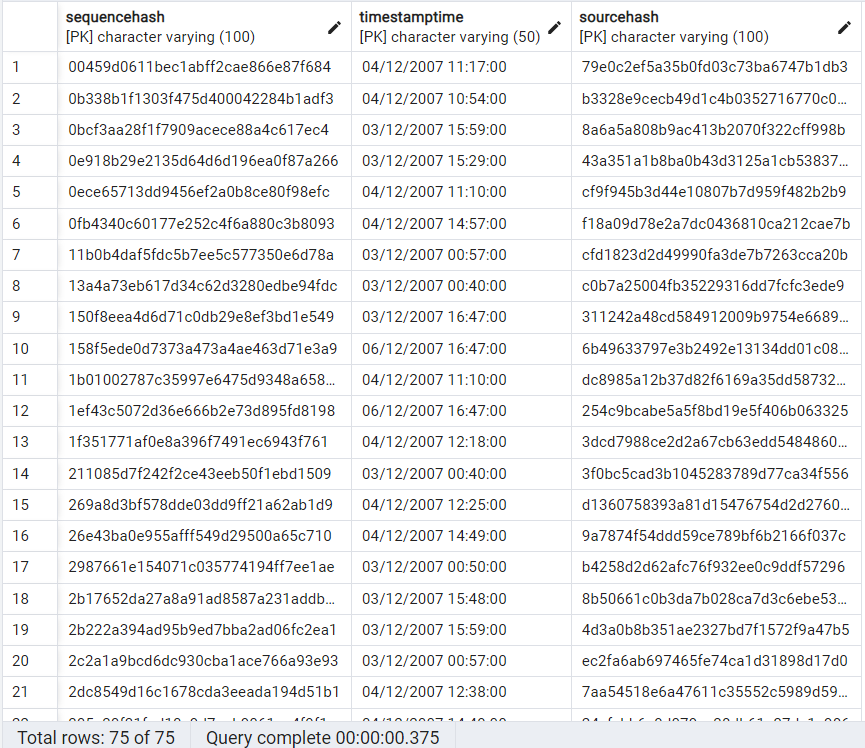
\includegraphics[width=0.7\linewidth]{experiment.png}}
	\caption{experiment result}
	\label{experiment}
\end{figure}
\begin{figure}[htbp]
	\centering{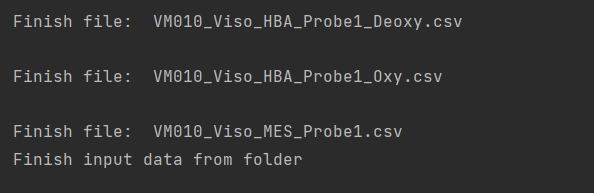
\includegraphics[width=0.7\linewidth]{finish.png}}
	\caption{Process}
	\label{finish}
\end{figure}
\hspace*{0.2cm} From the result, the project successfully finished enterprise layer and part of the staging and information mart layers.

\section{Discussion}
This session will discuss some solutions and own ideas for the problem during the production project.For the project function finish two part.
In Enterprise layer, finishing the data vault created which conform to concept and requirement of function. For the staging and information mart layers, which finished inserting the first data set, and processing the excel file and put it into the data vault\\
\subsection{Database}\label{AA}
The project do not use sql file and using '\textbackslash i' to create the database. Instead of common method this project uses the python to create the data vault. In python to connect SQL database and operate it has a powerful package named 'psycopg2'. The reason for choosing python is that when design the database in early stage, some details did not be considered very well, which means that the database will be modified as we process the data and planner can not guarantee that the database designed at the beginning of the project is good.If project use a SQL file and shell to create the database. The process for modifying the data vault is very tedious.In the end project decided to choose python to create the database directly; this is also for later maintenance and the continued development of the project considerations.
\\
For the Data vault design. Hubs have a primary key of a hash value, the time of data collection and the filename of the source as three values joint primary keys. The corresponding hash value is a foreign key in the satellite table. This makes it easier to find specific data in the future. A many-to-many relationship can be made clearer by storing the primary key of the associated hubs as foreign keys in the Link table.\\

\hspace*{0.2cm} The project uses three values as the joint primary key for the primary key. The sequence encodes the data as a hash to reduce the possibility of primary key conflicts. timestamp is when the data was collected to better manage the data in the future. Source hash marks the source of the data for future maintenance and management and is better protected by hashing the source. The hash of the source can be used to protect personal privacy.
\subsection{staging process}\label{AA}
In order to insert data into an already created data vault, the data in giving file needs to be split and combined into the fields and types that the database required to store.The project only excel type files can be read so here is an example of a 'csv' files. The files are combined by two parts. One is 'Header' and another is 'Data'. The header contains basic information about an experiment, group name, subjects, factor values, etc.\\
\hspace*{0.2cm} For the Header, the part involves the metadata of one experiment. By splitting the header data can get information about the experiment, such as the experimental group, subjects, and the factors influencing the experiment, which can be stored in the satellite tables of the data vault in accordance with the requirements of the database for future queries. For extracting data information, the project has created a special addressing function to find the keywords needed for the first project. Using python functions for file processing, the file is read line by line, and only the required values are removed from the metadata tags by cutting the characters.\\
\hspace*{0.2cm} The Data part after header involve values, times using etc. There is a column name for each column and the number of rows (index) so this data is used 'DataFrame' in pandas. The reason for using the Pandas package is that there is a very convenient way to read excel files directly and preserve the original formatting as much as possible. The 'DataFrame' structure also allows for the deletion of empty columns in the dataset.Allows the program to process data more efficiently.The data divides two part using time and values store in the observation tables as array.
\section{Conclusion}
This project has successfully created a data vault for medical imaging and has been proven feasible and effective by inserting data and theoretical refinements. The project was a success as the final results were very much in line with the final requirements.\\
\hspace*{0.2cm} However there are a number of areas for improvement in this project, the first of which is the limitation that the current project can only read files in excel format. However, the final structure of medical imaging data is only sometimes in excel format, so future work will need to expand the types of files the program can handle. Secondly, the database structure of the project is not comprehensive enough, and I believe that the data is stored in too many single locations. In the database design of this project, all the data, including the control and experimental groups, were stored in observation, but this will cause unnecessary problems for future queries, especially when the amount of data stored reaches a high level. This structure will hurt the efficiency of differentiating between experimental and control groups and make the whole query process very The entire query process is very cumbersome. The original form should be enhanced by adding a new hub ExperimentGroup and its corresponding satellite table to distinguish the experimental data from the control data and to improve its uniqueness.

\begin{thebibliography}{00}
\bibitem{b1} Linstedt, Dan (December 2010). Super Charge your Data Warehouse. Dan Linstedt. ISBN 978-0-9866757-1-3, pp. 74
\bibitem{b2} Linstedt, Dan (December 2010). Super Charge your Data Warehouse. Dan Linstedt. ISBN 978-0-9866757-1-3, pp. 74
\bibitem{b3} Denney, MJ (2016). "Validating the extract, transform, load process used to populate a large clinical research database". International Journal of Medical Informatics. 94: 271–4.
\bibitem{b4} What are hubs in Data Vault.[Online].Available: https://www.data-vault.co.uk/what-is-data-vault/
\bibitem{b5} What are Links in Data Vault.[Online].Available: https://www.data-vault.co.uk/what-is-data-vault/
\bibitem{b6} What are Satellites in Data Vault.[Online].Available: https://www.data-vault.co.uk/what-is-data-vault/
\bibitem{b7} README.rst[Online].Available:https://github.com/psycopg/psycopg2
\bibitem{b8} What is it[Online].Available:https://github.com/pandas-dev/pandas
\bibitem{b9} Chad R, Dougherty (31 December 2008). "Vulnerability Note VU836068 MD5 vulnerable to collision attacks"
\end{thebibliography}


\end{document}
